\documentclass[a4paper, 12pt]{article}
% Language setting
% Replace `english' with e.g. `spanish' to change the document language
\usepackage[english]{babel}

% Set page size and margins
% Replace `letterpaper' with `a4paper' for UK/EU standard size
%\usepackage[letterpaper,top=2cm,bottom=2cm,left=3cm,right=3cm,marginparwidth=1.75cm]{geometry}

% Useful packages
\usepackage{amsmath}
\usepackage{amssymb}
\usepackage{cite}  % merge citations more than one
\usepackage{graphicx}
\usepackage[usenames,dvipsnames]{color}
\graphicspath{{imgs/}}
\usepackage[colorlinks=true, allcolors=blue]{hyperref}
\usepackage{caption}
\usepackage{booktabs}
\usepackage{multirow}

\newcommand{\myfig}[1]{{\color{black}#1}}
\newcommand{\myeq}[2][e]{{\color{black}#1quation~(\ref{#2})}}
\newcommand{\mytab}[1]{{\color{black}#1}}
\newcommand{\mycite}[1]{{\color{black}\cite{#1}}}

\title{Paper Template}
\author{Chen Zhang, \dots}
\date{}

\begin{document}
\maketitle

\begin{abstract}
Abstract here
\end{abstract}

\section{sec1}

easy to make citation as \mycite{sung2021global}; and it is also available for \myfig{Figure~\ref{tag1}}, \mytab{Table~\ref{tag2}}, and \myeq{Log-likelihood}.\par

\begin{figure}[htbp]
	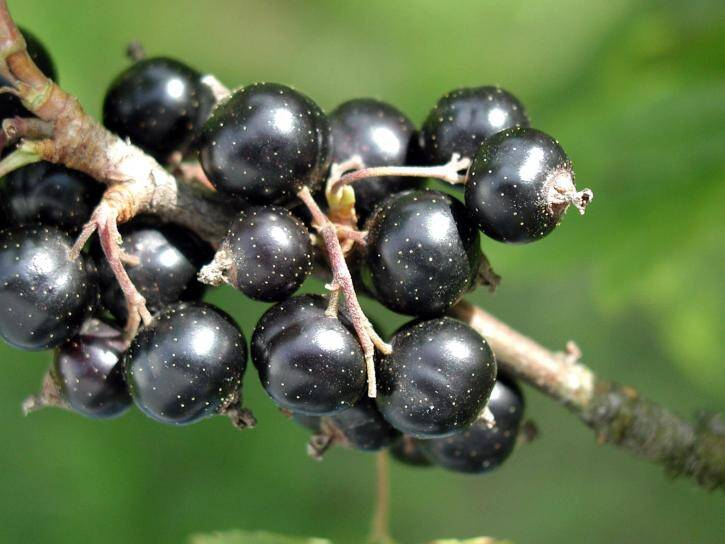
\includegraphics[scale=0.3]{blackcurrant.jpg}
	\caption{the blackcurrant}
	\label{tag1}
\end{figure}

\begin{table}[htbp]
    \begin{center}
    \caption{Example table}
    \begin{tabular}{c|c|c|c}
    \toprule
    Col1 & Col2 & Col2 & Col3 \\
    \midrule
    1 & 6 & 87837 & 787 \\ 
    \hline
    2 & 7 & 78 & 5415 \\
    \hline
    3 & 545 & 778 & 7507 \\
    \hline
    4 & 545 & 18744 & 7560 \\
    \hline
    5 & 88 & 788 & 6344 \\ [1ex] 
    \bottomrule
    \end{tabular}
    \label{tag2}
    \end{center}
\end{table}

\begin{align}\label{Log-likelihood}
\log L(\boldsymbol{\theta} | \boldsymbol{x}) &= \sum_{i \in 1:n} \log P(\boldsymbol{x} | \boldsymbol{\theta}) \nonumber \\
&= \sum_{i \in 1:n} \log \sum_{\boldsymbol{z}} P(\boldsymbol{x}, \boldsymbol{z} | \boldsymbol{\theta})
\end{align}

\clearpage
\bibliographystyle{unsrt}
\bibliography{paper}
\end{document}
